%%%%%%%%%%%%%%%%%%%%%%%%%%%%%%%%%%%%%%%%%%%%%%%%%%%%%%%%%%%%%%%%%%%
%                                                                 %
%                            CHAPTER ONE                          %
%                                                                 %
%%%%%%%%%%%%%%%%%%%%%%%%%%%%%%%%%%%%%%%%%%%%%%%%%%%%%%%%%%%%%%%%%%%

\chapter{INTRODUCTION}

\section{Definitions of Version} \label{sec:def}

Data sets invariably require versioning systems to manage changes due to an imperfect collection environment.
Data versioning systems are employed to manage changes to data, logging new data sets and communicating that change to data consumers.
Versioning discussion remains imprecise, lacking standardization or formal specifications.
Many works tend to define versions around examples and local characteristics but lack a broader foundation.
This work contributes to the discussion by capturing version relationships into a linked data model, taking inspiration from provenance models that incorporate versioning concepts such as PROV and Provenance, Authorship, Versioning (PAV) ontologies.

Using the term `version' in the vernacular has become so pervasive that few documents formally define it.
Barkstrom describes versions as \textbf{homogeneous groupings} used to control, ``production volatility induced by changes in algorithms and coefficients as result of validation and reprocessing," \cite{Barkstrom2003}.
The \textbf{groupings} he mentions are a method of separating data objects such that they have similar scientific or technical properties.
In order to determine when these properties have changed, he leverages the \gls{nasa} Earth Science workflow model shown in Figure \ref{NASALevels}.
\begin{figure}
	\centering
	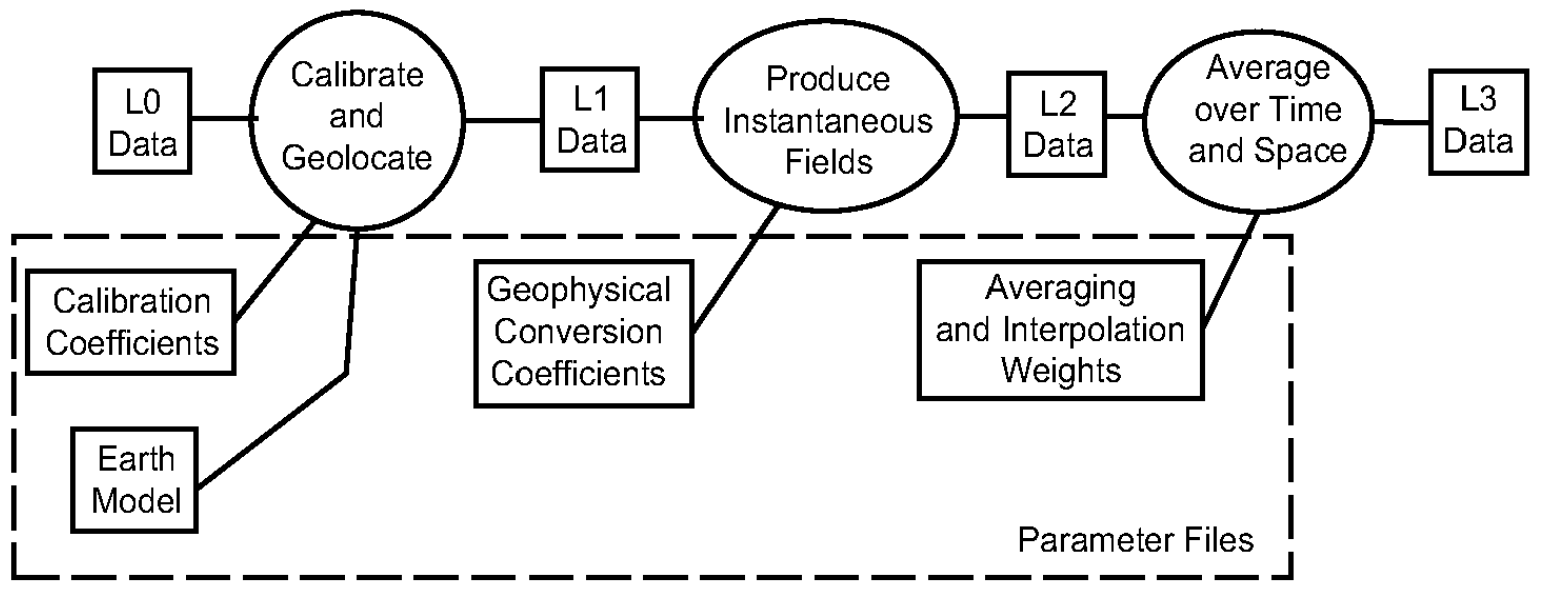
\includegraphics[scale=0.35]{figures/NASALevels.png}
	\caption[National Aeronautics and Space Administration Earth Science organizes its data into three levels depending on how much the data has been aggregated and processed from the original sensor measurements.]{National Aeronautics Space Administration Earth Science organizes its data into three levels depending on how much the data has been aggregated and processed from the original sensor measurements. Figure 1 from \cite{Barkstrom2003}}
	\label{NASALevels}
\end{figure}
The model describes the formal stages of processing to turn a raw remote sensing signal from satellite instruments into global aggregate summaries \cite{Barkstrom2003}.
The workflow model, therefore, describes a data object's \gls{provenance}, the information about how a piece of data or thing was created and used to determine its quality, reliability or trustworthiness \cite{Moreau2013c}, not the version differences.
Provenance provides the mechanism to explain differences between \textbf{groupings} exposed by versioning activities.
Understanding the workflow model reveals that changes to either the algorithms or parameter files will force a change in the resulting data, creating a new version of the output data.
Each time the provenance changes, the levels take on a layer cake appearance as shown in Figure \ref{NASALayers}. 
\begin{figure}
	\centering
	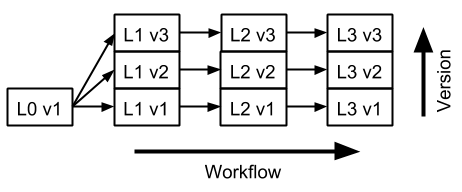
\includegraphics[scale=1]{figures/VersionLayerDiagram2.png}
	\caption[Versions Layered on the National Aeronautics and Space Administration Earth Science workflow model]{National Aeronautics and Space Administration Earth Science workflow model gains layers as changes to provenance induces version groupings to expand.  The new layer is homogeneous with other layers in the level, forming a grouping.  Level 0 cannot gain more layers because manipulating the source readings would invalidate the data.}
	\label{NASALayers}
\end{figure}
Unlike provenance, version information describes relations not along the workflow, but in an orthogonal direction because change passes through the layers.

The conflation can also be seen in \gls{linked} provenance models, Web of Data resources which describe the \gls{provenance} relating data sets, where version concepts and links are included into the ontology.
The \gls{prov} is the \gls{w3c} recommended method to document \gls{provenance}, connecting versions using the property \textit{prov:derivation}.
The \textit{prov:derivation}, covered more in Section \ref{sec:prov}, is defined as, ``a transformation of an entity into another, an update of an entity resulting in a new one, or the construction of a new entity based on a pre-existing entity," \cite{Lebo2013}.
The \gls{prov} definition establishes the existence of at least two distinct objects as a necessary condition for versioning.
An additional result of the \gls{prov} definition is that an object cannot be a version of itself.

Another definition comes from Tagger at University College London on versioning of biology data in which versions are a, ``semantically meaningful snapshot of a design object (an artifact) at a point in time," \cite{Tagger2005}.
He, unfortunately, does not further clarify what he means by semantically meaningful since the requirements to be meaningful varies based on the application.
He likely means that the design object must be complete or whole, interpretable in purpose by itself and not a subset.
The design object is used in the context of database objects, referring to an incomplete final product, and unifies the versions as their primary subject, capturing the object's state over the course of its design.

The \gls{ifla} formed a study group in February 1997 to, ``produce a framework that would provide a clear, precisely stated, and commonly shared understanding of what it is that the bibliographic record aims to provide information about, and what it is that we expect the record to achieve in
terms of answering user needs" \cite{frbr}.
A common problem in library sciences is the organization and documentation of multiple editions of a book or multiple translations of a book in a standardized manner.
A primary result of the group meeting is a standardized vocabulary to discuss distinct iterations of a literary work which follows strong parallels in data versioning.
The \gls{frbr} avoids the terms \textbf{edition} and \textbf{version} since ``those terms are neither clearly defined nor uniformly applied" \cite{frbr}.
Instead, they use the terms: \textbf{work}, \textbf{expression}, and \textbf{manifestation}.
A \textbf{work} refers to the abstract concept of a creative or artistic idea.
\textbf{Expressions} are then different forms of that particular \textbf{work}, embodying the most similar term to the previous definitions of versions.
A \textbf{manifestation} is the physical embodiment of an \textbf{expression}.
These three terms and their hierarchy establish a repeating theme throughout other versioning works.
The breakdown of terms identifies a need to differentiate between the granularity or scale of changes as differences in \textbf{works} are more significant than differences in \textbf{expressions}.
Models focused on versioning rather than provenance will also have a hierarchical structure as covered in Section \ref{sec:models}.

Combining these myriad of definitions, the Barkstrom definition provides the mechanism to detect and explain the source of a version.
The Tagger and \gls{prov} definitions explain the purpose of a version to expose differences between distinct objects.
The \gls{frbr} definition contextualizes a version as a more granular \textbf{expression} of a larger \textbf{work}.
The working definition in this dissertation of a \gls{version} is `an \textbf{expression} of a \textbf{work} which exists in comparison to another object and communicates the extent to which it diverges from that object as a result of provenance changes'.

Although each definition disagrees on the form a version object takes on, all but \gls{prov} derivation agree that a version belongs to a larger collection of objects implementing a more abstract, ideal representation.
Provenance provides the information necessary to explain ``semantically meaningful" for the Tagger definition as \textit{prov:Derivation} captures when a data object diverges into a new object.

\section{Why Versioning is Important}

\begin{quotation}
	``If scientific data production were easy, instruments would
	have stable calibrations and validation activities would discover no need for
	corrections that vary with time. Unfortunately, validation invariably shows that
	instrument calibrations drift and that algorithms need a better physical basis." \cite{Barkstrom2003}
\end{quotation}

Anyone who has used an iPhone or owned a video game console understands the basics of versioning.
Companies brand sequential devices to indicate improvements in performance or capabilities.
Basic numerical sequencing has given rise to a plethora of versioning systems used widely across a landscape of software and data.
At the very core, versioning systems are a means of communication.
Data producers communicate to consumers how much the producer has changed the data.
The producer can also communicate through time using logs and other documentation.
In order to clearly communicate changes, ideas must be clearly formalized and defined and vice versa.
Versioning systems help scientific workflows avoid losing work by managing transitions and changes while in operation \cite{Casati1996}.
Versioning systems provide necessary documentation which informs the transition to new methods and procedures \cite{Wiil:2000:RDH:338407.338517}.
Versioning systems provide accountability for the value of a project's data set when considering an agency's continued funding \cite{Cavanaugh2002}.
The natural evolution of versioning systems, however, have given rise to formal architecture operating on top of very informal concepts.
Disagreements between the informal concepts propagate through the formal architecture, causing breakdowns in interoperability between heterogeneous systems, especially when users are not aware of biases in informal versioning concepts \cite{Baker2009}.
In this dissertation, we identify gaps in versioning practices which result from tradition and develop a data model to more completely capture the interactions involved in versioning.

\subsection{Change Capture Completeness}

Data provenance has achieved major adoption and implementation goals in data management discussion with the adoption of PROV-O \cite{Lebo2013} as a \gls{w3c} recommendation and PROV-O's utilization in the \gls{nca} \cite{Ma2014191}.
The inclusion of versioning concepts within the ontology illustrates the close relationship between provenance and change information.
Provenance's prominence in the data management field defines a specific view of change capture.
Because provenance focuses on capturing the entities and activities used to produce a data object, it does not completely capture the change differences between objects.
Delving deeper and comparing the parts of the objects lies outside the scope of provenance information.
In order to achieve completeness, a \gls{linked} model must include the concepts of addition, invalidation, and modification.
The model must relate the changing parts which differentiate objects as separate versions with the objects.
The model must also maintain a continuity between versions to preserve the historical evolution of a data object.

\subsection{Change Log Performance}

A \gls{log} is a document explaining the differences between two versions \cite{uel1037}.
Every change logged within the \gls{log} requires a certain amount of storage space to document.
One of the ways to measure change log performance is to compute the number of entries in the change log relative to the space necessary to store the information.
The amount of change information generated for an object can be related to provenance information since changes to activities and inputs result in new data objects which can be compared to the original object as a version, generating change information.
Buneman finds that provenance data consumes storage space on the order of the original data, or after compression, the provenance takes up twenty percent of the original space \cite{Buneman}.
Including more data in a different form is guaranteed to decrease performance with the increased space utilization, but the reduction can be bounded.
Since the change log contains the differences between two versions, therefore containing at most all the entries in the data set, encoding the change data into the log will decrease performance by at most fifty percent.
The storage space necessary to hold the original change log and the change data is double the original data set size, but the entries remain the same since the change log and change data entries describe the same change.

\subsection{Change Distance Precision}

Versioning practices tend to follow specific traditions \cite{barkstrom2014earth}; one tradition is the use of dot-decimal identifiers to communicate change distance \cite{Tagger2005}.
A dot-decimal identifier is a series of numbers joined together by a decimal point with the left-most number signifying a grouping by major features and the right-most number signifying a grouping over the most minor features.
The amount of change between two versions is determined by finding the left-most interval at which the identifiers differ.
Because the identifiers traditionally denote a version's location in a sequence, only one interval is changed at a time and is only incremented by one.
The identifiers broadly categorize the change distance between two versions.
Because the number of changes between two versions is one or more, a range of change distances can fall within a category.
The range suggests that counting changes allows a more precise basis to report change distance than dot-decimal identifiers.

\subsection{Accuracy of Data Set Change Rate}

Looking at just the differences between versions may give a false impression of the data set's rate of change since the comparison to versions assumes that the versions are distributed evenly through time.
From Git \cite{Chacon:2009:PG:1618548} and other versioning systems \cite{Branco2008}, we can see versions can be arbitrarily distributed through time.
Variable publication rates help increase the stability of a project by controlling the data volatility, the likelihood of data to change, by aggregating changes before publishing a new version.
The division of changes across versions suggests that re-introducing time to change distance will give a more accurate reading of a data set's rate of change than the version publication rate and more accurate than changes across versions.

\section{Scope and Assumptions}

The data sets used to develop the versioning model include static tabular databases, taxonomic trees, and collections of small data sets possessing around twelve to thirteen files on average.
The static tabular databases contained on the order of thousands of records and the time between versions was on the order of months and years.
A number of classes of data do not reflect the temporal and size characteristics of the utilized data sets including streaming data, which posses short intervals between versions, and big-data repositories, which posses orders of magnitude more records.
Taxonomic trees do not represent many web ontologies because the ontologies may contain undirected cycles in the ontological structure.
The versioning model can only be applied to data sets with more than one version since the version must be compared to another object.

The model assumes that multiple changes occur between each version change.
The results in this thesis may not represent the performance of data sets which operate on single or small numbers of changes between each version of a data set.
Transactional data sets like centralized data sets are not covered by the research work in this thesis.
The model assumes that all newly appearing attributes have been added by the new version.
All attributes which do not appear in the new version are assumed to be invalidated.
The model assumes that every entry in a data set can be unique identified by an attribute or a combination of attributes.
Data sets where changes cannot be associated with mutually exclusive groups cannot be correctly represented in the versioning model.


\section{The Versioning Use Case} \label{sec:usecase}

The research questions addressed by this thesis revolve around the check and retrieval stages, steps 3 and 4a, of the flow in the Versioning Use Case shown in Table \ref{table:UseCase}.
\begin{table}
	\caption{Versioning Use Case Table}
	\label{table:UseCase}
	\centering
	\begin{tabular}{|L{14cm}|}
		\hline
		\textbf{Use Case Name}: New Version Publication \& Retrieval\\
		\hline
		\textbf{Goal}: Record a new version of a data set and provide it to a data consumer.\\
		\hline
		\textbf{Summary}: The Producer creates a new version of their data and must record it to the Versioning System while providing the Consumer with the data\\
		\hline
		\textbf{Actors}: Producer, Consumer\\
		\hline
		\textbf{Preconditions}: Producer has supplied some data to the Versioning System.   Consumer has retrieved the data from the Versioning System.\\
		\hline
		\textbf{Triggers}: Producer provides a different version of the data to the Versioning System.\\
		\hline
		\textbf{Basic Flow}: 
		\begin{enumerate}
			\item Producer places the next version into the Versioning System.
			\item Producer may repeat the previous action 0 or more times.
			\item Consumer checks the data to see if there are changes.
			\item If there are pertinent changes:
			\begin{enumerate}
				\item Consumer retrieves the updated data.
			\end{enumerate}
		\end{enumerate}\\
		\hline
		\textbf{Alternate Flow}:
		\begin{enumerate}
			\item Producer places the next version into the Versioning System.
			\item Producer notifies Consumer that an alternate version is available.
			\item Consumer retrieves the updated data.
		\end{enumerate}\\
		\hline
		\textbf{Post Conditions}: Producer has made the alternate version available.  Consumer possesses the pertinent newly available version.\\
		\hline
	\end{tabular}
\end{table}
The goal of the Versioning Use Case is to allow the Producer to communicate changes of data tracked by the versioning system to the Consumer.
The use case begins when a data producer wishes to distribute the next \gls{version} of a data set.
Note the use of next \gls{version} instead of new \gls{version} to signify that the Versioning Use Case also includes situations where the data is not new or describes concurrent events.
The use case features the Producer and Consumer as actors using the versioning system as an intermediary.
The actors do not follow separate use cases because each actor relies on the actions of the other actor to contextualize the actions in the use case.

The basic flow of the use case is seen in Figure \ref{UCD1} where the Producer logs a version into the versioning system, and the Consumer retrieves that data version.
\begin{figure}
	\centering
	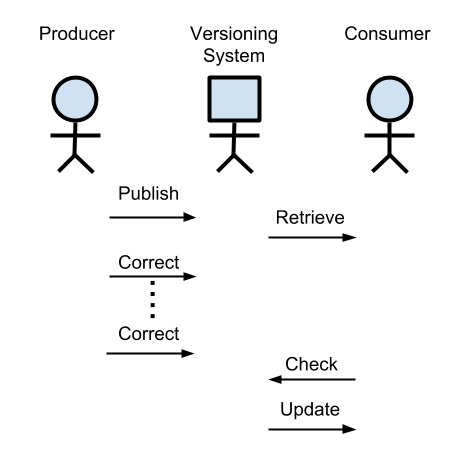
\includegraphics[scale=1]{figures/UC_Diagram1.png}
	\caption[Versioning Use Case Basic Flow]{Basic Flow of the Versioning Use Case.  The Producer adds a data set to be tracked by the versioning system.  After the Consumer retrieves the data, the Producer makes a series of updates and corrections to the original data.  The Consumer then returns to determine if there are changes to pertinent data files.  The Consumer then updates as necessary.}
	\label{UCD1}
\end{figure}
At a later point in time, the Producer can add any number of corrections to the versioning system.
The repeated corrections reflect a practice of passively logging additional changes.
At some final time after 0 or more corrections, the Consumer returns to check the versioning system for any changes to the data set the Consumer retrieved.
If there are changes to parts pertinent to the Consumer, the Consumer retrieves the corrected data.
In the interaction, the Producer only passively provides additional versions of the data while the responsibility of remaining up-to-date lies with the Consumer.
The ability of the  versioning system to communicate to the Consumer that the data has changed determines whether the use case succeeds or fails for the data consumer.
The relationship creates a Producer/Consumer dynamic which influences the performance of the versioning system.

The alternate flow in Figure \ref{UCD2} requires additional information from the Consumer which is a means of notification.
\begin{figure}
	\centering
	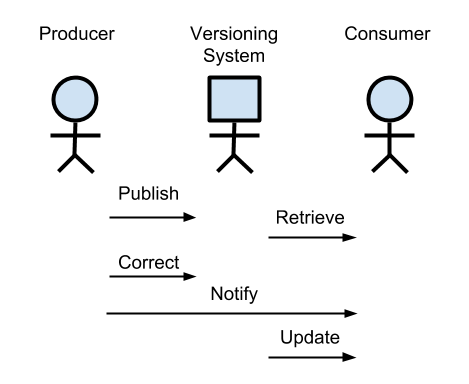
\includegraphics[scale=1]{figures/UC_Diagram2.png}
	\caption[Versioning Use Case Alternate Flow]{In the alternate flow, the authority to determine necessary updates lies with the Producer.  After correcting data tracked by the versioning system, the Producer notifies the Consumer to update the Consumer's data.}
	\label{UCD2}
\end{figure}
The flow begins the same as the basic flow, but after a single correction, the Producer notifies the Consumer that the data has changed.
The notification causes the Consumer to come and retrieve the updated data set.
The alternate flow poses a few problems in that the Producer must now manage notification information, but the Producer must also notify all consumers of the data which may cause scalability issues.
Notice that in both flows, the Producer possesses the authority to determine change through data publication.
The Consumer only takes from the versioning system except in step three of the basic flow.
It is only when the Consumer checks the \glspl{version} in the system or is notified by the Producer that the Consumer can contextualize changes to the retrieved data set.

\subsection{Research Question 1: What has changed?}

The primary research question addressed in the following chapters pertains to step three in the basic flow of the use case.
In order to execute step three, the Consumer must have a means of determining whether the data set is different from the one the Consumer currently possesses.
In a large number of software projects, especially open-source projects, \glspl{log} document for the Producer changes to the code base and communicate alterations to the Consumer.
Very few data sets provide detailed \glspl{log} along with \glspl{version} in the versioning system.
Either general descriptions of changes are made or new documentation explaining usage is provided, requiring the data consumer to manually acclimate to changes.

The prevailing approach to addressing Research Question 1 is that automating the generation of \glspl{log} will allow the addition of \gls{linked} into \gls{log} content.
To encode changes as \gls{linked}, I developed a versioning ontology called \gls{vo}.
The additional data allows data consumers the ability to search, filter, and otherwise interact with change information.
Different standards exist across various national agencies, but few fundamentals have been established on what needs to be included and how the information is to be captured or presented.
I determine whether a \gls{linked} versioning model would provide a standardized basis for discussing version change as well as allow tools to be developed to assist in step three for large data sets of which Consumers may only use a part.

\subsection{Research Question 2: How much has changed?}

A follow-up query to Research Question 1 is that once the changes have been determined, Consumers need to evaluate the impact of the changes.
As previously mentioned, Producers sequentially label \glspl{version} to communicate change, but many have adopted the practice of using decimals or dots to imply fractional changes, forming a dot-decimal identifier.
The authority to determine the magnitude of change lies with the Producer since the label must be applied at publication.
Version counts, defined in Chapter \ref{ch:graph}, provide a very bland description of the changes in a version by aggregating a range of changes under a sequential label.
Using \gls{vo}, the changes can be broken down into \gls{AIM} classifications which provide a quantitative method to determine \gls{changedist}.
I test whether the AIM change counts would tie change metrics back to data differences rather than to versions.
I determine whether the AIM changes also provide a means to compare the difference between the amount of change declared by the Producer and quantity of change as seen by various Consumers.

\subsection{Research Question 3: How fast does the data change?}

Once a standardized metric for determining \gls{changedist} has been determined, assessing change rate logically follows.
Up to this point, evaluating the differences between versions has been discussed without respect to time.
Notice from the Versioning Use Case that the Producer has the ability to control the rate of version release by determining when to push corrections into the versioning system, meaning the time between \glspl{version} is not required to be consistent.
Variable release times allows the Producer to control the data volatility, the likelihood of a data set to change, by aggregating changes over time.
Without considering time, \gls{changedist} across \glspl{version} misrepresents the actual change rate of a data set.
Looking at just the version publication rate also misrepresents the actual change rate of a data set since total change can vary between \glspl{version}.
I hypothesize that version analysis must factor in time when comparing change rates between \glspl{version}.
The change rate distribution of each \gls{AIM} \gls{change} follows a distribution significantly different from the version publication rate.

\section{Hypothesis Statement}

The work in this dissertation tests five hypotheses.
\begin{enumerate}
	\item \gls{vo}, compared to current provenance ontologies, increases the completeness of change graphs by capturing \gls{AIM} changes.
	\item \gls{vo} reduces performance of change logs by no more than 50\% where performance is measured by content per unit storage.
	\item \gls{vo} increases the precision and detail of change measurements compared to dot-decimal identifiers by enumerating changes.
	\item VersOn, compared to the version publication rate, increases the accuracy of capturing the data set change rate.
\end{enumerate}

\section{Contributions}

%Add chapter number and references.

In Chapter \ref{ch:model}, I present my first contribution, the model forming the basis of \gls{vo} which is used to instantiate \glspl{vergraph}.
\Glspl{vergraph} capture differences between objects, not the course used to create a data object, differentiating themselves from provenance graphs.
The \gls{vergraph} enables my second contribution, a structured process to compute and publish \gls{linked} \glspl{log} to test Hypothesis 1, covered in Chapter \ref{ch:changelog}.
The contribution eases consuming very lengthy logs, which data sets often produce, as well as enabling searchability and discoverability of \glspl{change} affecting the \gls{version}.
My third contribution, discussed in Chapter \ref{ch:graph}, is using a \gls{vergraph} to provide a quantitative metric for determining \gls{changedist}, a necessary component to answer Hypothesis 2.
Differing methods between data producers and consumers in computing \gls{changedist} highlights disagreements in the prodcuer/consumer dynamic which is demonstrated while evaluating Hypothesis 3.
A fourth contribution is a comparison between version publication and change rates, found in Chapter \ref{Volatility}, to determine the propriety of versions as proxies for change, used to test Hypothesis 4 and 5.

%%% Local Variables:
%%% mode: latex
%%% TeX-master: t
%%% End:
